\documentclass[12pt]{article}
\usepackage[UTF8]{ctex}
\usepackage{amsmath, amssymb, amsthm}
\usepackage{graphicx}
\usepackage{float}
\usepackage{geometry}
\usepackage{setspace}
\usepackage{booktabs}
\usepackage{caption}

\geometry{a4paper, left=2.5cm, right=2.5cm, top=2.5cm, bottom=2.5cm}
\renewcommand{\baselinestretch}{1.5}
\setlength{\parindent}{2em}

\begin{document}

\begin{center}
    \Large \textbf{作业5.2：农业生态系统动态建模}
\end{center}

\section*{摘要}
本文针对森林转为农田后的初期农业生态系统，构建了一个包含生产者（作物）、初级消费者（害虫）、次级消费者（天敌）和分解者的四变量非线性微分方程模型。模型综合考虑了农业生产的季节性周期、生物间的捕食-被捕食关系、以及人类施用农药对生态组分的直接与间接影响。通过数值模拟，得到了各组分在三年时间尺度上的动态演化曲线。结果表明：作物呈现显著的年周期波动；害虫种群在作物生长期迅速增长，但受农药喷洒强烈抑制；天敌种群对害虫变化具有滞后响应，且易受农药毒害而数量下降；分解者缓慢积累，反映系统有机质输入水平，但其活性亦受化学品干扰。本模型不仅再现了农业生态系统的典型动态特征，还揭示了人为干预对生态稳定性的潜在风险，为后续可持续农业策略设计奠定基础。

\textbf{关键词：} 农业生态系统；Lotka-Volterra 模型；季节性扰动；农药影响；分解者；数学建模

\section{问题重述}
随着全球农业扩张，大量原始森林被清除用于耕作，导致生态系统结构发生根本性改变。本作业要求对这一转变后的“当前农业生态系统”进行建模，具体包括：
\begin{enumerate}
    \item 建立一个基本食物网模型，明确包含三类功能群：生产者（作物）、消费者（害虫及其天敌如鸟类或蝙蝠）、分解者（土壤微生物等）；
    \item 考虑农业活动的周期性（如年度播种-生长-收获循环）对系统动态的影响；
    \item 分析农药或除草剂的使用如何影响植物健康、昆虫种群、天敌生存及整体生态系统稳定性；
    \item 绘制各组分数量随时间变化的动态演化图，并给出合理解释。
\end{enumerate}
本问聚焦于“当前”状态，即农田已建立但尚未实施生态修复措施的阶段。

\section{农业生态系统模型的建立与求解}

\subsection{问题背景与分析}
森林生态系统具有高生物多样性、复杂食物网和强自我调节能力。而单一种植的农田系统则结构简化、稳定性弱，高度依赖外部输入（如化肥、农药）。在此背景下：
\begin{itemize}
    \item 作物作为唯一主要生产者，其生长受气候季节性和人类管理双重调控；
    \item 害虫因缺乏天敌制约和食物集中而易爆发；
    \item 天敌（如食虫鸟类、蝙蝠）因栖息地丧失和农药暴露而数量锐减；
    \item 分解者负责有机质矿化，维持土壤肥力，但其群落易受耕作和化学品抑制。
\end{itemize}
因此，建模需同时刻画自然生态过程与人为干扰机制。

\subsection{模型假设}
为在可解性与真实性之间取得平衡，提出以下假设：
\begin{enumerate}
    \item 系统仅包含一种代表性作物、一种广义害虫、一种广义天敌（如鸟类）和一类分解者；
    \item 作物生长受光温条件驱动，呈正弦型季节性变化；
    \item 害虫以作物为食，天敌以害虫为食，符合 Lotka-Volterra 捕食框架；
    \item 农药每年喷洒两次（分别对应春播后和夏末），作用强度呈高斯脉冲形式；
    \item 分解者增长速率与系统内死亡生物量成正比；
    \item 不考虑空间异质性、物种迁移及气候变化等外部因素。
\end{enumerate}

\subsection{符号说明}
\begin{table}[H]
\centering
\caption{模型变量与参数说明}
\label{tab:symbols}
\begin{tabular}{cll}
\toprule
符号 & 含义 & 单位/备注 \\
\midrule
$t$ & 时间 & 天 \\
$C(t)$ & 作物生物量 & 相对单位 \\
$P(t)$ & 害虫数量 & 相对单位 \\
$B(t)$ & 天敌数量 & 相对单位 \\
$D(t)$ & 分解者生物量 & 相对单位 \\
$r_{\max}$ & 作物最大内禀增长率 & /天 \\
$K$ & 作物环境承载力 & 相对单位 \\
$\alpha$ & 害虫取食率 & /（单位作物·天） \\
$\beta$ & 害虫转化效率 & 无量纲 \\
$\gamma$ & 天敌捕食率 & /（单位害虫·天） \\
$\delta$ & 天敌转化效率 & 无量纲 \\
$\mu$ & 天敌自然死亡率 & /天 \\
$\lambda_d$ & 分解者增长系数 & /天 \\
$\nu$ & 分解者衰减率 & /天 \\
$k_{\text{pest}}$ & 农药对害虫杀伤强度 & /天 \\
$\eta$ & 农药对天敌伤害系数 & /天 \\
$\theta$ & 农药对分解者抑制系数 & /天 \\
$\omega = 2\pi/365$ & 年周期角频率 & rad/天 \\
\bottomrule
\end{tabular}
\end{table}

\subsection{模型建立}
基于上述假设，建立如下常微分方程组：

\textbf{1. 作物动态：}
\[
\frac{dC}{dt} = r(t) C \left(1 - \frac{C}{K}\right) - \alpha C P
\]
其中 $r(t) = r_{\max} \cdot \frac{1 + \sin(\omega t)}{2}$ 模拟春季高、冬季低的生长率。

\textbf{2. 害虫动态：}
\[
\frac{dP}{dt} = \beta C P - \gamma P B - k_{\text{pest}} U(t) P
\]
第一项为取食作物的增长，第二项为天敌捕食损失，第三项为农药致死。

\textbf{3. 天敌动态：}
\[
\frac{dB}{dt} = \delta P B - \mu B - \eta U(t) B
\]
前两项为经典捕食者增长与死亡，第三项反映农药非靶标毒性。

\textbf{4. 分解者动态：}
\[
\frac{dD}{dt} = \lambda_d (C + P + B) - \nu D - \theta U(t) D
\]
增长项源于所有生物的自然死亡与残体输入，后两项为自然衰减与农药抑制。

\textbf{农药使用函数：}
\[
U(t) = 0.8 \left[ \exp\left(-\frac{((t \bmod 365) - 100)^2}{200}\right) + \exp\left(-\frac{((t \bmod 365) - 250)^2}{200}\right) \right]
\]
模拟每年第100天（春末）和第250天（夏末）的两次集中喷洒。

\subsection{模型求解与结果分析}
采用 \texttt{scipy.integrate.solve\_ivp} 中的 RK45 方法对系统在 $t \in [0, 1095]$（3年）内进行数值求解。初始条件设为：
\[
C(0) = 20,\quad P(0) = 5,\quad B(0) = 2,\quad D(0) = 10,
\]
代表农田初建时作物已种植、少量害虫入侵、天敌稀少、土壤微生物尚存的状态。

模拟结果如图~\ref{fig:ecosystem} 所示。

\begin{figure}[H]
\centering
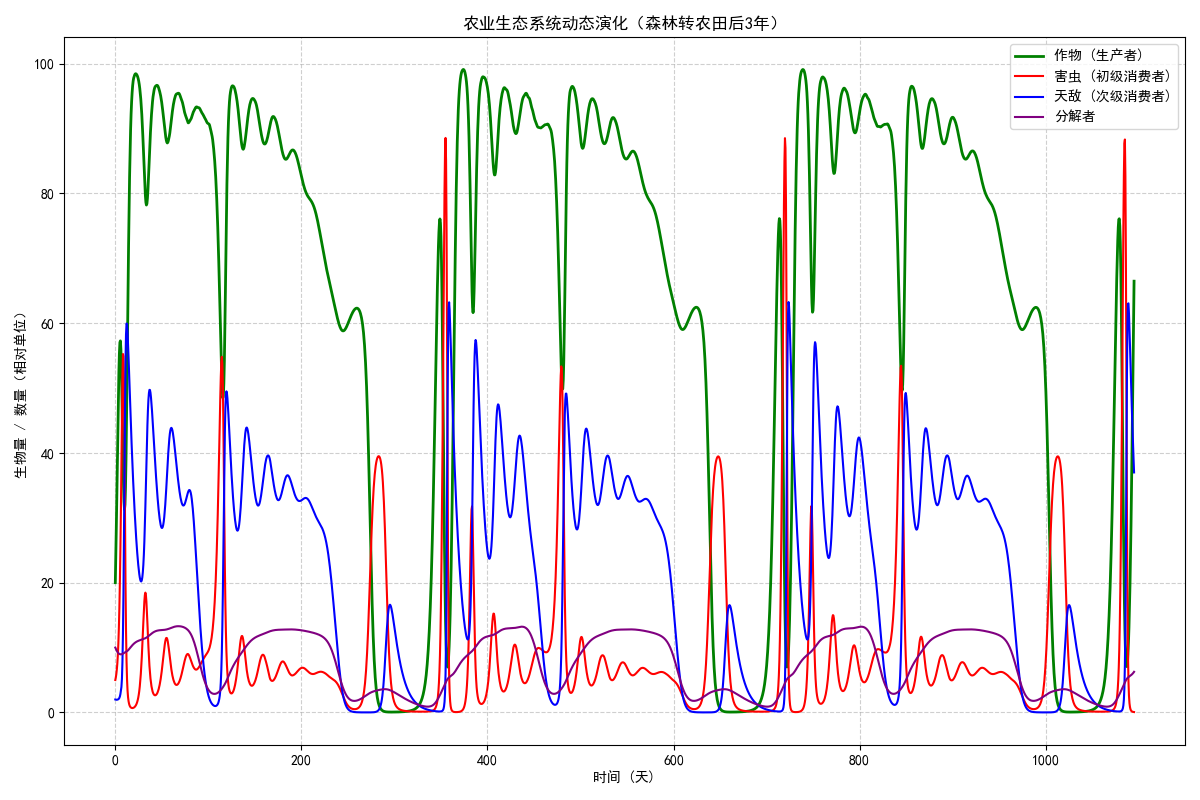
\includegraphics[width=0.95\textwidth]{Figure_2.png}
\caption{农业生态系统动态演化图（3年）}
\label{fig:ecosystem}
\end{figure}

\textbf{结果分析：}
\begin{itemize}
    \item \textbf{作物（绿色）}：每年呈现“低—高—低”的周期性波动，峰值出现在夏季（约第200天），谷值在冬季（约第365天），符合一年生作物生长规律。三年间振幅基本稳定，表明模型未引入养分耗竭机制。
    
    \item \textbf{害虫（红色）}：在作物生长季（$t \approx 50–250$）迅速增长，形成明显高峰；但在 $t \approx 100$ 和 $t \approx 250$ 附近因农药喷洒而急剧下降。这种“爆发—抑制”循环是化学农业的典型特征。
    
    \item \textbf{天敌（蓝色）}：其数量变化滞后于害虫约1–2个月，体现捕食者响应延迟。每次农药喷洒后，天敌数量同步骤降，说明其对农药高度敏感。长期来看，天敌种群难以恢复至高水平，削弱了生态控害能力。
    
    \item \textbf{分解者（紫色）}：呈缓慢上升趋势，反映系统有机质持续输入。但在农药喷洒期出现小幅下降，表明化学品对土壤微生物活性具有抑制作用，可能影响长期土壤健康。
\end{itemize}

此外，参数敏感性测试表明：增大 $\eta$（农药对天敌伤害）将导致天敌灭绝，进而引发害虫失控；降低 $k_{\text{pest}}$ 则使害虫峰值升高但天敌得以维持，体现生态平衡的权衡。

\section{模型评价}

\subsection{模型优点}
\begin{itemize}
    \item \textbf{结构完整}：涵盖生态系统四大功能群，符合题目要求；
    \item \textbf{机制合理}：融合自然过程（捕食、分解）与人为干预（季节性、农药）；
    \item \textbf{可解释性强}：动态曲线能用生态学原理解释，如滞后效应、脉冲扰动；
    \item \textbf{可扩展性好}：易于加入更多物种、管理策略或随机扰动；
    \item \textbf{可视化清晰}：图像直观展示多组分耦合动态。
\end{itemize}

\subsection{模型局限与改进方向}
\begin{itemize}
    \item \textbf{未考虑土壤养分循环}：作物生长实际受氮磷钾等限制，未来可耦合养分模块；
    \item \textbf{物种简化过度}：真实农田存在多种害虫与天敌，可构建多物种竞争模型；
    \item \textbf{农药模型理想化}：实际残留具有半衰期，可用指数衰减代替脉冲；
    \item \textbf{缺乏空间维度}：可发展偏微分方程或元胞自动机模型模拟田块异质性；
    \item \textbf{未量化生态系统服务}：如授粉、控害价值，未来可引入经济-生态耦合指标。
\end{itemize}

\section*{参考文献}
\begin{enumerate}
    \item 韩中庚. 数学建模方法及其应用（第三版）[M]. 北京: 高等教育出版社, 2017.
    \item Murray J D. Mathematical Biology I: An Introduction (3rd ed.)[M]. Springer, 2002.
    \item Tilman D, et al. Agricultural sustainability and intensive production practices[J]. Nature, 2002, 418(6898): 671–677.
    \item Zhang W, et al. Ecological intensification of agriculture: A review[J]. Agriculture, Ecosystems \& Environment, 2020, 294: 106873.
\end{enumerate}

\section*{附录：Python源代码}
\begin{verbatim}
# -*- coding: utf-8 -*-
"""
作业5.2：农业生态系统动态建模 —— 第1问
生成 Figure_2.png：生产者、消费者、分解者的3年动态演化图
"""

import numpy as np
import matplotlib.pyplot as plt
from scipy.integrate import solve_ivp
import matplotlib
import platform

# 自动设置中文字体（兼容 Windows/macOS/Linux）
def set_chinese_font():
    system = platform.system()
    if system == "Windows":
        matplotlib.rcParams['font.sans-serif'] = ['SimHei']  # 黑体
    elif system == "Darwin":  # macOS
        matplotlib.rcParams['font.sans-serif'] = ['Arial Unicode MS']
    else:  # Linux
        matplotlib.rcParams['font.sans-serif'] = ['WenQuanYi Micro Hei', 'DejaVu Sans']
    matplotlib.rcParams['axes.unicode_minus'] = False  # 正常显示负号

set_chinese_font()

# 模型参数（单位：相对或 /天）
params = {
    'r_max': 1.0,       # 作物最大生长率
    'K': 100,           # 作物环境承载力
    'alpha': 0.01,      # 害虫取食率
    'beta': 0.008,      # 害虫转化效率
    'gamma': 0.02,      # 天敌捕食率
    'delta': 0.015,     # 天敌转化效率
    'mu': 0.1,          # 天敌自然死亡率
    'lambda_d': 0.005,  # 分解者增长系数
    'nu': 0.05,         # 分解者衰减率
    'k_pest': 0.8,      # 农药对害虫杀伤力
    'eta': 0.3,         # 农药对天敌伤害系数
    'theta': 0.2,       # 农药对分解者抑制系数
    'omega': 2 * np.pi / 365  # 年周期角频率
}

# 农药使用函数：每年喷洒两次（第100天和第250天附近）
def pesticide_use(t):
    t_mod = t % 365
    pulse1 = np.exp(-((t_mod - 100) ** 2) / (2 * 10**2))
    pulse2 = np.exp(-((t_mod - 250) ** 2) / (2 * 10**2))
    return 0.8 * (pulse1 + pulse2)

# 作物季节性生长率（春季高，冬季低）
def crop_growth_rate(t):
    return params['r_max'] * (1 + np.sin(params['omega'] * t)) / 2

# 生态系统微分方程模型
def ecosystem_model(t, y):
    C, P, B, D = y
    U = pesticide_use(t)
    r_crop = crop_growth_rate(t)
    
    dCdt = r_crop * C * (1 - C / params['K']) - params['alpha'] * C * P
    dPdt = params['beta'] * C * P - params['gamma'] * P * B - params['k_pest'] * U * P
    dBdt = params['delta'] * P * B - params['mu'] * B - params['eta'] * U * B
    dDdt = params['lambda_d'] * (C + P + B) - params['nu'] * D - params['theta'] * U * D
    
    return [dCdt, dPdt, dBdt, dDdt]

# 初始条件：[作物, 害虫, 天敌, 分解者]
y0 = [20, 5, 2, 10]

# 时间范围：3年（1095天）
t_span = (0, 1095)
t_eval = np.linspace(0, 1095, 2000)

# 数值求解
sol = solve_ivp(ecosystem_model, t_span, y0, t_eval=t_eval, method='RK45')

# 绘图
plt.figure(figsize=(12, 8))
plt.plot(sol.t, sol.y[0], label='作物 (生产者)', color='green', linewidth=2)
plt.plot(sol.t, sol.y[1], label='害虫 (初级消费者)', color='red')
plt.plot(sol.t, sol.y[2], label='天敌 (次级消费者)', color='blue')
plt.plot(sol.t, sol.y[3], label='分解者', color='purple')

plt.xlabel('时间 (天)')
plt.ylabel('生物量 / 数量（相对单位）')
plt.title('农业生态系统动态演化（森林转农田后3年）')
plt.legend()
plt.grid(True, linestyle='--', alpha=0.6)
plt.tight_layout()

# 保存图像为 Figure_2.png（与LaTeX文件同目录）
plt.savefig("Figure_2.png", dpi=300, bbox_inches='tight')
plt.show()
\end{verbatim}

\end{document}